\chapter{结构}
\label{chp:structure}

\begin{quotation}
善张网者引其纲,不一一摄万目而后得。
\begin{flushright}
--- 《韩非子·外储说右下》
\end{flushright}
\end{quotation}

在 \ref{sec:structure} 节中我们曾简略提及文档的结构,本章将对它们展开介绍。通常一篇文档无论长短都会有标题和正文。如果正文较长,有个层次结构会便于行文,阅读起来也较方便。为了便于查找,长文档通常会前有目录,后有索引。另外为了便于编辑,长文档通常会被分割成多个文件。和 HTML 类似,PDF 也提供超链接功能,它也放在本章介绍。学术文档一般还会有参考文献,以供读者参考、借鉴。

以上诸项通常会按标题、目录、正文、参考文献、索引这样的顺序出现。如果是正式出版的书籍,还会有标题页、版权页、献辞页等;而且这些结构出现的奇偶页也有讲究,比如版权页是偶数页,目录首页是奇数页。同学们若对书籍的格式装帧有兴趣,可以参考 Peter R. Wilson\indexWilson{} \footnote{剑桥大学机械学士,诺丁汉大学半导体物理博士。本科毕业后就职于不列颠托马森休斯顿公司 (British Thomson Houston) ;后跳到卢卡斯研究中心 (Lucas Research Center) 搞 CAD,曾任计算机辅助制造国际 (Computer-Aided Manufacturing International, CAM-I) 欧洲分部主席;再到 GE 参与开发 CAD/CAM 数据交换标准 STEP;又到RPI, 美国天主教大学 (Catholic University of America), 国家标准技术研究所 (National Institute of Standards and Technology, NIST) 等院所从事科研,最后从波音退休。} 的\emph{Notes on Book Design}\citep{Wilson_memdesign}和\emph{Memoir Class}\citep{Wilson_memoir},或者\emph{Chicago Manual of Style}\citep{Chicago_style}。

\section{长文档}

文章想要吸引读者就必须写得好,想要影响深远就必须写得长。包子曰:神奇卓异非至人,至人只是长。当文档很长时,我们最好把它分为多个文件,各个击破,从而缓解长期伏案写作带来的悲观厌世情绪。这和高速公路上为了防止疲劳驾驶设置的技术弯道有异曲同工之妙。

\autoref{exa:include} 示范了如何在主控文档中引用子文档。注意 \verb|\include| 命令会新起一页,如果不想要新页可以改用 \verb|\input| 命令。

\begin{example}[htbp]
\begin{Code}[]
%master.tex
\begin{document}
\include{chapter1.tex}
\include{chapter2.tex}
...
\end{document}
\end{Code}
\caption{拆分长文档}
\label{exa:include}
\end{example}

当文档很长时,编译一遍也会很花时间。我们可以使用 \verb|syntonly| 宏包,这样编译时就只检查语法,而不生成结果文件。

\begin{Code}[numbers=none]
\usepackage{syntonly}
...
\syntaxonly
\end{Code}

\section{标题}

在 \autoref{exa:title} 中,我们用 \verb|\title|, \verb|\author|, \verb|\date| 等命令分别设置标题、作者、日期。标准文档类没有为作者所属单位定义专门的命令,我们可以把单位直接写在作者下面,作者和单位之间的联系通常用一些特殊符号来标注。设置上述内容之后,我们用 \verb|\maketitle| 命令来输出它们。

\autoref{tab:class_options} 中提到的文档类选项 \texttt{notitlepage} 和 \texttt{titlepage} 可以用来控制标题是否单独占一页。 \texttt{report} 和 \texttt{book} 文档类中的标题缺省独占一页,\texttt{article} 文档类中的标题缺省和正文等混居一页。

\begin{example}[h]
\begin{Code}[]
\title{`雷人的传说`}
\author{`包太雷`$^*$\quad `包巨雷`$^\dagger$\quad 
  `包最雷`$^\ddagger$\\[10pt]
$*$Barrington University, Burlington, VT\\
$\dagger$Pacific Western University, San Diego, CA\\
$\ddagger$Preston University, Los Angeles, CA}
\date{2011`年`1`月`11`日`}
\maketitle
\end{Code}
\begin{Demo}
\centering
\includegraphics[page=4,scale=1]{mini.pdf}
\end{Demo}
\caption{标题}
\label{exa:title}
\end{example}

\section{目录}

\verb|\tableofcontents| 命令可以用来生成整个文档的章节目录。\LaTeX 会自动设定目录包含的章节层次,我们也可以用 \verb|\setcounter| 命令来指定目录的层次深度。如果不想让某个章节标题出现在目录里,则可以使用 \autoref{exa:toc} 中带 \texttt{*} 的命令来声明章节。

\begin{example}[!h]
\begin{Code}[]
\tableofcontents
\setcounter{tocdepth}{2}
\chapter*{...}
\section*{...}
\subsection*{...}
\end{Code}
\caption{目录}
\label{exa:toc}
\end{example}

类似地,我们可以使用 \verb|\listoffigures| 和 \verb|\listoftables| 命令来生成图目录和表目录。

当章节或图表等结构发生变化时,我们需要执行两次编译命令以获得正确的目录。其中第一次编译生成一些中间文件,后缀分别为 \texttt{.toc} (目录), \texttt{.lof} (图目录), \texttt{.lot} (表目录) ;第二次编译则把这些中间文件和其他内容整合起来。\LaTeX 之所以设计成这样可能是因为当时的电脑内存容量有限。

另外我们也可以利用 Axel Sommerfeldt\indexSommerfeldt 的 \texttt{caption} 宏包\citep{Sommerfeldt_caption}来自定义类似于插图和表格的浮动环境。本文中的例子浮动环境就是用 \autoref{exa:float} 中的方法生成的,第2行代码指定 \texttt{loe}为例目录中间文件后缀,\texttt{example} 为环境名,\texttt{例}为浮动环境标题前缀,\texttt{例目录}是目录的标题。定义该环境后,其使用方法与插图、表格浮动环境一样,见第3--5行。

\noindent
\verb|语法:\DeclareCaptionType[选项]{环境}[名称][目录名]|
\begin{example}[htbp]
\begin{Code}[numbers=none]
\usepackage{caption}
\DeclareCaptionType[fileext=loe]{example}[`例`][`例目录`]
\begin{example}[htbp]
...
\end{example}
\end{Code}
\caption{自定义浮动环境}
\label{exa:float}
\end{example}

\section{参考文献}

\subsection{\texttt{thebibliography}}
\label{sec:thebibliography}

在学术文档中人们经常要用到参考文献 (bibliography) ,这样做既可以有选择地提供事实,作客观公证科学严谨状,还可以拉帮结派党同伐异。

\LaTeX 中最原始的方法是用 
\texttt{thebibliography} 环境和 \verb|\bibitem| 命令来定义参考文献条目。在 \autoref{exa:thebibliography} 中,第1行的参数 \texttt{9} 是参考文献条目编号的宽度;如果有几十个条目,可以把该参数改为 \texttt{99}。

\begin{example}[htbp]
\begin{BTDemo}[]
\begin{thebibliography}{9}
\bibitem{Rowling_1997}
  Joanne K. Rowling,
  \emph{Harry Potter and the Philosopher's Stone}.
  Bloomsbury, London,
  1997.
\end{thebibliography}
\end{BTDemo}
\caption{\texttt{thebibliography} 环境}
\label{exa:thebibliography}
\end{example}

\texttt{thebibliography} 环境一般放在文档的末尾。定义了参考文献之后,我们可以用 \verb|\cite| 命令在正文中引用条目。

\begin{RLDemo}[numbers=none]
\cite{Rowling_1997}
\end{RLDemo}

\subsection{BibTeX}

\texttt{thebibliography} 环境的一个缺点是,用户得自己调整显示格式,这样做很麻烦而且易出错。

Oren Patashnik (1954--)\indexPatashnik{} \footnote{1976年毕业于耶鲁,1990年斯坦福 Knuth 门下电脑博士。1980年加入贝尔实验室。} 和 Lamport\indexLamport 就在1985年想出一个办法,用数据库文件 \texttt{.bib} 记录参考文献条目,用样式文件 \texttt{.bst} 设置显示格式。普通用户一般不需要改动 样式文件,只需维护数据库。

这种方法秉承了 \LaTeX 内容与格式分离的思想,我们在 SGML/DSSSL, HTML/CSS, XML/XSL 等技术上也可以见到同样的思路。

\BibTeX 将参考文献分为十几种类型,每种类型的参考文献有不同的必选项和可选项 (见以下列表) 。

\begin{compactdesc}
  \item [article] 期刊或杂志上的文章
    \begin{compactitem}
      \item 必选项:author, title, journal, year
      \item 可选项:volume, number, pages, month, note
    \end{compactitem}
  \item [conference] 同inproceedings
  \item [book] 正式出版的书籍
    \begin{compactitem}
      \item 必选项:author/editor, title, publisher, year
      \item 可选项:volume/number, series, address, edition, month, note
    \end{compactitem}
  \item [booklet] 非正式出版的小册子
    \begin{compactitem}
      \item 必选项:title
      \item 可选项:author, howpublished, address, month, year, note
    \end{compactitem}
  \item [inbook] 书的一部分,比如章、节,或某些页
    \begin{compactitem}
      \item 必选项:author/editor, title, chapter/pages, publisher, year
      \item 可选项:volume/number, series, type, address, edition, month, note
    \end{compactitem}
  \item [incollection] 书中比较独立的一部分
    \begin{compactitem}
      \item 必选项: author, title, booktitle, publisher, year 
      \item 可选项:editor, volume/number, series, type, chapter, pages, address, edition, month, note
    \end{compactitem}
  \item [inproceedings] 会议论文
    \begin{compactitem}
      \item 必选项:author, title, booktitle, year
      \item 可选项:editor, volume/number, series, pages, address, month,  organization, publisher, note.
    \end{compactitem}
  \item [manual] 手册
    \begin{compactitem}
      \item 必选项: title
      \item 可选项:author, organization, address, edition, month, year, note
    \end{compactitem}
  \item [mastersthesis] 硕士论文
    \begin{compactitem}
      \item 必选项:author, title, school, year
      \item 可选项:type, address, month, note
    \end{compactitem}
  \item [misc] 实在不好分类时只好用它
    \begin{compactitem}
      \item 必选项:无
      \item 可选项:author, title, howpublished, month, year, note
    \end{compactitem}
  \item [phdthesis] 博士论文
    \begin{compactitem}
      \item 必选项:author, title, school, year
      \item 可选项:type, address, month, note
    \end{compactitem}
  \item [proceedings] 会议论文集
    \begin{compactitem}
      \item 必选项:title, year
      \item 可选项:editor, volume/number, series, address, month, organization, publisher, note
    \end{compactitem}
  \item [techreport] 技术报告
    \begin{compactitem}
      \item 必选项:author, title, institution, year
      \item 可选项:type, number, address, month, note
    \end{compactitem}
  \item [unpublished] 未出版文档
    \begin{compactitem}
      \item 必选项:author, title, note
      \item 可选项:month, year
    \end{compactitem}
\end{compactdesc}

编辑 \texttt{.bib} 文件时可以用普通文本编辑器,也可以用专门的文献管理软件来
提高效率,后者包老师推荐 JabRef。一些其他的文献管理软件或网络服务也可以输出 \texttt{.bib} 格式,比如 EndNote, Google Scholar, Zotero 等。

\autoref{exa:thebibliography} 中罗琳阿姨的书可以用 \BibTeX 改写成 \autoref{exa:bibtex} 中的样子。其中每行是一个数据项,第一个数据项是关键字,供引用时用;其他数据项都以 \texttt{名称=值} 的形式成对出现,值要写在双引号之内;数据项之间用逗号分隔。

\begin{example}[htbp]
\begin{Code}[]
@book{Rowling_1997,
  author    = "Joanne K. Rowling",
  title     = "Harry Potter and the Sorcerer's Stone",
  publisher = "Bloomsbury, London",
  year      = "1997"
}
\end{Code}
\caption{\BibTeX 数据}
\label{exa:bibtex}
\end{example}

有了数据后,我们需要选一个样式。通常的 \LaTeX 发行版都会带有四种标准的样式,如果觉得这些标准格式无法满足你的需要,可以参考 Nicolas Markey (1976--)\indexMarkey{} \footnote{1994年数学学士,1998年巴黎第七大学 (Paris Diderot University) 数学和电脑双硕士,2003年奥尔良大学 (University of Orléans) 电脑博士。布鲁塞尔自由大学博士后,2004年加入 CNSR。} 的《野兽调教》\citep{Markey_beast}。

\begin{compactdesc}
  \item [plain] 参考文献列表按作者姓氏排序,序号为阿拉伯数字。
  \item [unsrt] 参考文献列表按正文中引用顺序排序,序号为阿拉伯数字。
  \item [alpha] 参考文献列表按作者姓氏排序,序号为作者姓氏加年份。
  \item [abbrv] 类似 \texttt{plain} 样式,作者名字、月份、期刊名等用缩写。
\end{compactdesc}

选定样式后,我们需要在文档中用 \verb|\bibliographystyle| 命令来设置样式,然后用 \verb|\bibliography| 命令输出参考文献列表。

\begin{Code}[numbers=none]
\bibliographystyle{plain}
\bibliography{myref}
\end{Code}

前文中我们提到含有交叉引用的文档需要编译两遍。含有参考文献的文档更麻烦,它需要依次执行四次编译操作。

\begin{enumerate}
  \item 第一遍 \texttt{xelatex} 把参考文献条目的关键字写到中间文件 \texttt{.aux}  里去。
  \item \texttt{bibtex} 根据 \texttt{.aux, .bib, .bst} 生成一个 \texttt{.bbl}  文件,即参考文献列表。它的内容就是 \texttt{thebibliography} 环境和一些 \verb|\bibitem| 命令。
  \item 第二遍 \texttt{xelatex} 把交叉引用写到 \texttt{.aux} 中去。
  \item 第三遍 \texttt{xelatex} 则在正文中正确地显示引用。
\end{enumerate}

\begin{figure}[htbp]
\centering
\includegraphics[page=22]{pgf.pdf}
\caption{\BibTeX 的编译}
\label{fig:bibtex}
\end{figure}

有多个子文档时,我们可以在每个子文档中用 \verb|\bibliographystyle| 命令设置不同的样式;当然如果没有特别的理由,包老师还是建议用统一的样式。编译时用 \texttt{xelatex} 编译主控文档,而用 \texttt{bibtex} 编译各个子文档。

\begin{example}[htbp]
\begin{Code}[numbers=left]
xelatex master(.tex)
bibtex chapter1(.tex)
bibtex chapter2(.tex)
...
xelatex master(.tex)
xelatex master(.tex)
\end{Code}
\caption{子文档参考文献的编译}
\label{exa:subdoc_bibtex}
\end{example}

\subsection{Natbib}

参考文献在正文中的引用通常有两种模式:作者-年份和数字。\LaTeX 提供的 \verb|\cite| 命令只支持数字模式,Patrick W. Daly\indexDaly{} \footnote{马克斯·普朗克太阳系研究所 (Max Planck Institute for Solar System Research) 研究员。} 的 \texttt{natbib} 宏包\citep{Daly_natbib}则同时支持这两种模式。

\texttt{natbib} 提供了三种列表样式:\texttt{plainnat, abbrvnat, unsrtnat},它们的参考文献列表和相对应的 \LaTeX 标准样式 \texttt{plain, abbrv, unsrt} 效果相同,只是在引用时可以自由选择作者-年份或数字模式。

这两种模式以及他一些细节的设置 (比如标点符号) 在本文中被称作引用样式。\texttt{natbib} 的三种列表样式都有自己的缺省引用样式,如要定制引用样式,可以使用 \verb|\setcitestyle| 命令;其选项见 \autoref{tab:citestyle},其中上标模式其实就是把数字标号移到了上标位置。

\begin{table}[htbp]
\caption{参考文献引用样式选项}
\label{tab:citestyle}
\centering
\begin{tabular}{ll}
  \toprule
  引用模式            & authoryear, numbers, super \\
  括号                & round, square, open={char}, close={char} \\
  引用条目分隔符      & 分号, 逗号, citesep={char} \\
  作者年份分隔符      & aysep={char} \\
  共同作者年份分隔符  & yysep={char} \\
  注解分隔符          & notesep={text} \\
  \bottomrule
\end{tabular}
\end{table}

\texttt{natbib} 提供了多种引用命令,其中最基本的是 \verb|\citet| 和 \verb|\citep|,它们在不同引用模式下效果不同。一般不推荐使用 \LaTeX 本身提供的 \verb|\cite| 命令,因为它在作者-年份模式下和 \verb|\citet| 效果相同,在数字模式下和 \verb|\citep| 相同。这些模式下引用命令的效果见 \autoref{exa:cite} 。

\begin{example}[htbp]
\begin{RLDemo}[numbers=none]
\setcitestyle{authoryear}
see \cite{Daly_natbib}\\
see \citet{Daly_natbib}\\
see \citep{Daly_natbib}
\end{RLDemo}

\begin{RLDemo}[numbers=none]
\setcitestyle{numbers}
see \cite{Daly_natbib}\\
see \citet{Daly_natbib}\\
see \citep{Daly_natbib}
\end{RLDemo}

\begin{RLDemo}[numbers=none]
\setcitestyle{super}
see \cite{Daly_natbib}\\
see \citet{Daly_natbib}\\
see \citep{Daly_natbib}
\end{RLDemo}
\caption{各种引用模式下的引用命令效果}
\label{exa:cite}
\end{example}

另外还有一些引用命令,如 \verb|\citetext|, \verb|\citenum|, \verb|\citeauthor|, \verb|\citeyear| 等,读者可以自行查阅手册,此处不赘述。

\section{索引}

\texttt{makeidx} 宏包提供了索引功能。应用它时,我们首先要在文档序言部分引用宏包,并使用 \verb|\makeindex| 命令;其次在正文中需要索引的地方定义索引,注意索引关键字在全文中须保持唯一;最后在合适的地方 (一般是文档末尾) 打印索引。

\begin{example}[htbp]
\begin{Code}[]
\usepackage{makeidx}
\makeindex
...
\begin{document}
\index{`索引关键字`}
...
\printindex
\end{document}
\end{Code}
\caption{索引}
\label{exa:index}
\end{example}

当编译含索引的文档时,用户需要执行三次编译操作,

\begin{compactenum}
  \item 第一遍 \texttt{xelatex} 把索引条目写到一个 \texttt{.idx} 文件中去。
  \item \texttt{makeindex} 把 \texttt{.idx} 排序后写到一个 \texttt{.ind} 文件中去。
  \item 第二遍 \texttt{xelatex} 在 \verb|\printindex| 命令的地方引用 \texttt{.ind} 的内容,生成正确的文档。
\end{compactenum}

\begin{figure}[htbp]
\centering
\includegraphics[page=23]{pgf.pdf}
\caption{索引的编译}
\label{fig:index}
\end{figure}

\section{超链接}
\label{sec:hyperlink}

Rahtz\indexRahtz 和 Heiko Oberdiek\indexOberdiek{} \footnote{pdfTeX 开发者之一,几十个宏包的作者。} 的 \texttt{hyperref} 宏包\citep{Rahtz_hyperref}提供了一些超链接功能。它给文档内部的交叉引用和参考文献自动加上了超链接,还提供了其他几个命令。

\verb|\hyperref| 命令对已经定义的标签进行简单包装,加上文字描述。

\begin{example}[htbp]
\LoadFBTDemo[]{texlet/hyperref}
\caption{\texttt{\char`\\hyperref} 命令}
\label{exa:hyperref}
\end{example}

\verb|\url| 和 \verb|\href| 命令可以用来定义外部链接,后者有文字描述。

\begin{example}[htbp]
\LoadFBTDemo[numbers=none]{texlet/href}
\caption{\texttt{\char`\\url} 和 \texttt{\char`\\href} 命令}
\label{exa:href}
\end{example}

\section{结构名}

在 \LaTeX 中,每个文档结构都有自己的名字,一般用来在标题中或引用时显示。比如主目录、图目录、表目录的名字分别是:Contents, List of Figures, List of Tables;章、节、小节的名字分别是:Chapter, Section, Subsection;图和表的名字是 Figure 和 Table。

\autoref{exa:structure_name} 列出了标准文档类中定义的结构名变量,其中 \verb|\bibname| 是 \texttt{book} 文档类的专有变量;\verb|\abstractname| 和 \verb|\refname| 是 \texttt{report} 和 \texttt{article} 文档类专有的;其他变量对这三种文档类都适用。

如果我们想改变这些变量的值,比如中文文档需要中文结构名,可以用 \autoref{exa:structure_name} 中的方法来重定义这些结构名变量。例中第4, 5行代码是为了顺应中文的习惯。

\begin{example}[htbp]
\begin{Code}[]
\renewcommand{\contentsname}{`目录`}
\renewcommand{\listfigurename}{`图目录`}
\renewcommand{\listtablename}{`表目录`}
\renewcommand{\partname}{`第` \thepart `部分`}
\renewcommand{\chaptername}{`第` \thechapter `章`}
\renewcommand{\figurename}{`图`}
\renewcommand{\tablename}{`表`}
\renewcommand{\bibname}{`参考文献`}
\renewcommand{\appendixname}{`附录`}
\renewcommand{\indexname}{`索引`}
\renewcommand{\abstractname}{`摘要`}
\renewcommand{\refname}{`参考文献`}
\end{Code}
\caption{标准文档类结构名重定义}
\label{exa:structure_name}
\end{example}

\ref{sec:crossref} 节中提到的 \verb|\ref| 命令显示的是数字。\texttt{hyperref} 宏包提供了一个 \verb|\autoref| 命令,它可以自动判断标签所属结构对象的类型,为引用加上合适的名字,输出时显示结构名加上结构编号。该宏包也为此定义了一些结构变量名,我们也可以用同样的方法重定义它们 (见 \autoref{exa:autoref_name}) 。

\begin{example}[htbp]
\begin{Code}[]
\renewcommand{\equationautorefname}{`公式`}
\renewcommand{\footnoteautorefname}{`脚注`}
\renewcommand{\itemautorefname}{`项`}
\renewcommand{\figureautorefname}{`图`}
\renewcommand{\tableautorefname}{`表`}
\renewcommand{\appendixautorefname}{`附录`}
\renewcommand{\theoremautorefname}{`定理`}
\end{Code}
\caption{\texttt{hyperref} 宏包结构名重定义}
\label{exa:autoref_name}
\end{example}

需要注意的是,\verb|\autoref| 命令输出的结果总是名称在编号前面,对于章、节等结构无法产生“第x章”、“第x节”等符合中文习惯的结果。所以 \autoref{exa:autoref_name} 略去了若干这样的结构名,我们在引用时需要手工在 \verb|\ref| 命令前后加上合适的字眼。

%hyperref选项

\bibliographystyle{unsrtnat}
\bibliography{lnotes2}
